\subsection{Definiciones y propiedades básicas}

Un anillo es una estructura algebraica que cuenta con dos operaciones internas, a diferencia de los grupos, que solo cuentan con una. En el contexto de un anillo, a la primera de estas operaciones se le llama \emph{suma}, y a la segunda, \emph{multiplicación}. En ese sentido, usaremos los símbolos <<$+$>> y <<$\cdot$>> para referirnos a ellas, a pesar de que la naturaleza de estas operaciones puede ser muy distinta dependiendo del anillo concreto en el que estemos trabajando.

\begin{definition}[Anillo, anillo conmutativo, identidad]
    Un \emph{anillo} es una terna $(R, +, \cdot)$, donde $R$ es un conjunto y $+ \colon R \times R \to R$ y $\cdot \colon R \times R \to R$ son funciones (totales) que satisfacen los siguientes axiomas:\footnote{Algunos autores 
    no incluyen el axioma $3$ en la definición de anillo, y usan el término \emph{anillo con identidad} para referirse a la estructura algebraica que nosotros llamamos simplemente \emph{anillo}. No hay una convención universal sobre esto, por lo que sugerimos siempre revisar la definición precisa de anillo en el material que se esté utilizando.}
    \begin{enumerate}
        \item $(R, +)$ es un grupo abeliano.
        \item $\cdot$ es asociativa: para todos $a,b,c \in R$ se cumple que $(a \cdot b) \cdot c = a \cdot (b
\cdot c)$.

	\item Existe un elemento $\1 \in R$ (llamado \emph{identidad}) tal que para todo $a \in R$ se cumple que $a \cdot \1 = \1 \cdot a = a$

   \item $\cdot$ distribuye sobre $+$, es decir, para todos $a, b, c \in R$ se cumple que $a \cdot (b + c) = (a \cdot b) + (a \cdot c)$ y $(a+b) \cdot c = (a \cdot c ) + (b \cdot c).$
    \end{enumerate}
    Decimos que $(R, +, \cdot)$ es un \emph{anillo conmutativo} si es un anillo en el que la operación $\cdot$ es conmutativa.\hfill$\blacksquare$
    \end{definition}

Notemos que el axioma $4$ es el único que conecta ambas operaciones, y lo hace de la misma manera en que interactúan la suma y multiplicación usuales.

En el apéndice de teoría de grupos discutimos que el símbolo $e$ estaba siempre reservado para el neutro. Sin embargo, en el contexto de un anillo, usaremos el símbolo $\0$ para referirnos al neutro de la operación $+$. La letra negrita sirve para diferenciar dicho elemento del número $0$. Siempre usaremos la notación aditiva para el grupo $(R, +$), de modo que $-a \in R$ denotará al inverso de $a \in R$ bajo $+$. En la misma línea, dados $a \in R$ y $n \in \mathbb{Z}$, escribiremos $na$ para denotar a la $n$-ésima potencia de $a$ bajo $+$.

También usaremos la negrita para diferenciar el elemento $\1 \in R$ del número $1$. Para que esta notación tenga sentido, primero debemos probar que la identidad de un anillo es única. La demostración es idéntica a la que hicimos para grupos.

\begin{proposition}
    La identidad de un anillo es única.
\end{proposition}
    
    \begin{proof}
    Sea $(R, +, \cdot)$ un anillo, y supongamos que $\1, \1' \in R$ son ambos identidades. Como $\1$ es identidad, tenemos que $\1 \cdot \1' = \1'$. Pero $\1'$ también es identidad, así que $\1 \cdot \1' = \1$. Por transitividad, concluimos que $\1 = \1'$.
    \end{proof}

Dado un $a \in R$ y un entero positivo $n$, escribiremos $a^n$ para denotar al elemento $a$ operado bajo $\cdot$ consigo mismo $n$ veces. También definimos $a^0 = \1$. Notemos que, \textit{a priori}, no tiene sentido escribir $a^n$ si $n$ es un entero negativo, pues podría no existir un inverso para $a$ bajo $\cdot$.

Con el objetivo de no sobrecargar la notación, es usual omitir el símbolo <<$\cdot$>> para escribir multiplicaciones. Además, a menos que un par de paréntesis indique lo contrario, la convención es que la multiplicación tiene mayor prioridad que la suma. Así, los axiomas de distributividad se suelen escribir como $a(b+c) = ab+ac$ y $(a+b)c = ac + bc$. 

Nos centraremos en el estudio de los anillos conmutativos, pues no necesitaremos trabajar con ningún anillo no conmutativo en este documento.

\begin{example} 
Sabemos que $(\mathbb{Z}, +)$ es un grupo abeliano (ejemplo \ref{ejemplo_Z}). Si consideramos además la multiplicación usual de enteros, obtenemos el anillo conmutativo $(\mathbb{Z}, +, \cdot)$. \hfill$\blacksquare$
\end{example}

\begin{example}
Dado un entero $n \geq 1$, sabemos que $(\mathbb{Z}_n, +)$ es un grupo abeliano (ejemplo \ref{grupo_ciclico}). Si consideramos además la multiplicación usual en módulo $n$, obtenemos un anillo conmutativo: $(\mathbb{Z}_n, +, \cdot)$. \hfill$\blacksquare$
\end{example}

A continuación presentamos algunas propiedades básicas de los anillos conmutativos.

\begin{proposition}[Propiedad absorbente del neutro aditivo] \label{propiedad absorbente}
    Sea $(R, +, \cdot)$ un anillo conmutativo y $a \in R$ un elemento cualquiera. Entonces se cumple que $a\cdot \0 =\0\cdot a= \0$.
\end{proposition}

\begin{proof}
Sabemos que $\0+\0 = \0$, pues $\0$ es el neutro aditivo. Luego:
    \begin{eqnarray*}
\0+\0 = \0		&\Rightarrow & a\cdot(\0+\0) = a\cdot \0\\
        &\Rightarrow &a\cdot \0+a\cdot \0 = a\cdot \0.
    \end{eqnarray*}
Como $(R, +)$ es un grupo abeliano, podemos cancelar $a \cdot \0$ (proposición \ref{cancelacion_grupos}). Así, obtenemos que $a \cdot \0 = \0$. Por la conmutatividad de la multiplicación, también tenemos que $\0 \cdot a=\0 $.
\end{proof}

\begin{remark} \label{obs_cero_distinto_a_uno}
    La proposición \ref{propiedad absorbente} muestra que si en un anillo conmutativo $(R, +, \cdot)$ se cumple que $\0 = \1$, entonces $R$ tiene un solo elemento. En efecto, si eso se cumple, entonces para todo $a \in R$ se tendrá que
    $$a = a \cdot \1 = a \cdot \0 = \0.$$
    Por lo tanto, el único anillo conmutativo en el que se cumple que $\0 = \1$ es la estructura trivial. En el caso de los cuerpos (definición \ref{definicion_cuerpo}) uno agrega la condición $\0 \neq \1$ para evitar tener que analizar ese caso por separado.
    \hfill$\blacksquare$
\end{remark}

\begin{proposition}\label{propiedades_anillos}
    Sea $(R, +, \cdot)$ un anillo conmutativo. Se cumplen las siguientes propiedades:
    \begin{enumerate}
    \item Para todos $a,b\in R$ se cumple que $(-a)\cdot b=-(a\cdot b) = a\cdot (-b)$.
    
    \item Para todos $a \in R$ y $n \in \mathbb{Z}$ se cumple que $-(na) = (-n)a = n(-a)$.
    
    \item Para todo $a \in R$ y $n,m \in \mathbb{Z}$ se cumple que $(nm)a = n(ma)$.
    
    \item Para todos $a,b\in R$ y $n \in \mathbb{Z}$ se cumple que $n(a\cdot b) = (na)\cdot b = a \cdot (nb)$. De esto y la propiedad 4 se concluye que, para todo $a,b\in R$ y $n,m \in \mathbb{Z}$, se cumple que $(nm)(a\cdot b) = (na)\cdot (mb)$.   
    \end{enumerate}
    \end{proposition}
    
    \begin{proof} \hfill
        \begin{enumerate}
        \item Tenemos que:
            \begin{eqnarray*} (-a)\cdot b + a \cdot b & = & ((-a) +
            a) \cdot b\\ & = & \0 \cdot b\\ 
            & = & \0 \quad\quad\quad \text{por la propiedad absorbente del $\0$}.
            \end{eqnarray*}
    Luego $-(a \cdot b) = (-a)\cdot b$. Usando esto y la 
            conmutatividad de la multiplicación, obtenemos que $$a\cdot (-b) = (-b) \cdot a = -(b\cdot a) = -(a\cdot b).$$
    
            \item Si $n = 0$, entonces $-(na) = (-n)a = n(-a) = \0$ por definición de la notación $kc$ (para $k \in \mathbb{Z}$ y $c \in
            R$). Si $n > 0$, tenemos que $(-n)a = n(-a)$ por definición. Por otro lado, se cumple que
    \begin{eqnarray*}
    (-n)a + na & = & n(-a) + na\\
    & = & \underbrace{(-a) +\cdots + (-a)}_\text{$n$ veces} \ + \ \underbrace{a +\cdots + a}_\text{$n$ veces}\\ 
    & = & \underbrace{((-a) + a) + \cdots + ((-a) + a)}_\text{$n$ veces}\\
    & = & \underbrace{\0 + \cdots + \0}_\text{$n$ veces}\\
    & = & \0.
    \end{eqnarray*}
    Luego $-(na) = (-n)a$. Dejamos el caso $n < 0$ como ejercicio para el lector (para resolverlo es útil considerar el caso $n > 0$ y la propiedad $n = -|n|$). 
    
    \item Si $n = 0$ o $m = 0$, entonces $(nm)a = n(ma) = \0$ por definición de la notación $kc$ (para $k \in \mathbb{Z}$ y $c \in
            R$). Si $n > 0$ y $m > 0$, tenemos que
    \begin{eqnarray*}
    (nm)a &=& \underbrace{a +\cdots + a}_\text{$nm$ veces}\\
     &=& \underbrace{c +\cdots + c}_\text{$n$ veces} \quad\quad\quad \text{para }
     c = \underbrace{a +\cdots + a}_\text{$m$ veces}\\
     & = & \underbrace{ma +\cdots + ma}_\text{$n$ veces}\\
     & = & n(ma).
    \end{eqnarray*}
    Si $n < 0$ y $m < 0$, entonces $-n > 0$ y $-m > 0$, y podemos usar el caso que acabamos de probar:
    \begin{eqnarray*}
    (nm)a &=& ((-n)(-m))a\\
     &=& (-n)((-m)a)\\
     &=& (-n)(-(ma)) \quad\quad\quad \text{por la propiedad 2}\\
     &=& n(-(-(ma))) \quad\quad\quad \text{por la propiedad 2}\\
     &=& n(ma)
    \end{eqnarray*}
    Los casos faltantes son análogos: los dejados como ejercicios para el lector.
    
        \item Si $n = 0$, tenemos que $n(a\cdot b) = (na)\cdot b = a \cdot (nb)$ por la propiedad absorbente del $\0$ y la definición de la notación $kc$ (para $k \in \mathbb{Z}$ y $c \in F$). Si $n > 0$, tenemos que:
        \begin{eqnarray*}
            n(a\cdot b)&=&\underbrace{a\cdot b +\cdots + a\cdot b}_\text{$n$ veces}\\
            &=&(\underbrace{a +\cdots + a}_\text{$n$ veces}) \cdot b\\
            &=&(na) \cdot b
        \end{eqnarray*}		
    Utilizando esta propiedad y la conmutatividad de la multiplicación, obtenemos que $$n(a\cdot b) = n(b \cdot a) = (nb) \cdot a = a \cdot (nb).$$ Si $n < 0$, entonces 
    $n = -|n|$ con $|n| > 0$. Utilizando el caso que acabamos de probar, tenemos que
        \begin{eqnarray*}
            n(a\cdot b)&=& (-|n|)(a \cdot b)\\
            &=& |n|(-(a \cdot b))\\
            &=& |n|((-a) \cdot b) \quad\quad\quad \text{por la propiedad 1}\\
            &=& (|n|(-a)) \cdot b\\
            &=& ((-|n|)(a)) \cdot b\\
            &=& (na) \cdot b
        \end{eqnarray*}
        Finalmente, utilizando eso y la conmutatividad de la multiplicación obtenemos $n(a\cdot b) = a \cdot (nb)$. 
        \qedhere
        \end{enumerate}
    \end{proof}

También hay una noción de isomorfismo para anillos, que veremos a continuación.

\begin{definition}[Isomorfismo de anillos]
    Sean $(R_1, +_1, \circ_1)$ y $(R_2, +_2, \circ_2)$ dos anillos. Diremos que una función $\phi\colon R_1 \rightarrow R_2$ es un \emph{isomorfismo} si $\phi$ es una biyección y, además,
    $$\forall\, a, b \in R_1 \qquad \phi(a +_1 b) = \phi(a) +_2 \phi(b) \quad \land \quad \phi(a \circ_1 b) = \phi(a) \circ_2 \phi(b).$$
    Si existe un isomorfismo, se dice que los anillos $R_1$ y $R_2$ son \emph{isomorfos}, y se escribe $R_1 \simeq R_2$. \hfill$\blacksquare$
    \end{definition}
    
    En otras palabras, un isomorfismo es una biyección entre los anillos que también induce una biyección entre las relaciones definidas por las operaciones binarias. 
    Al igual que en el caso de grupos, no es difícil convencerse de que dos anillos isomorfos tienen exactamente las misma propiedades. Por ejemplo, si $R_1 \simeq R_2$, entonces $R_1$ es conmutativo si y solo si $R_2$ es conmutativo.


En general, en un anillo no tenemos la propiedad de cancelación para la multiplicación. Veamos el siguiente ejemplo.

\begin{example} \label{ejemplo_no_dominio_integral}
Consideremos el anillo $(\mathbb{Z}_6,+,\cdot)$. Si
queremos resolver la ecuación $$ 2\cdot x\ = \ 4,$$ no podemos
``cancelar'' el $2$ en ambos lados de la ecuación y concluir que $x =
2$. De hecho, si bien $x =2$ es una raíz de la ecuación, también lo es $x=5$, ya que $2 \cdot 5 = 4$ en módulo $6$. El problema aquí es que $2$ no tiene inverso multiplicativo en este anillo, por lo que no es correcto deducir que $x=2$ a partir de la ecuación $ 2\cdot x\ = \ 4$. Notemos que se cumplen las siguientes equivalencias:
$$2 \cdot x = 4 \quad
 \Leftrightarrow \quad 2 \cdot x - 4 = 0 \quad \Leftrightarrow \quad 2 \cdot (x - 2) = 0.$$
Por lo tanto, necesitamos que $2 \cdot (x-2)$ sea congruente a $0$ en módulo $6$. Si bien esto es cierto cuando $x=2$, también lo es cuando $x=5$, en cuyo caso el producto queda $2 \cdot 3 = 0$ (ya que $6$ es congruente a $0$ en módulo $6$). Esto muestra que en un anillo es posible multiplicar dos elementos distintos al $\0$ y obtener el $\0$, algo que no ocurre con los números reales. En general, el anillo $(\mathbb{Z}_n,+,\cdot)$, con $n \geq 2$ un número compuesto, tendrá el mismo problema: existirán elementos $a\neq 0$ y $b\neq 0$
tales que $a\cdot b = 0$.
 \hfill$\blacksquare$
\end{example}

El ejemplo \ref{ejemplo_no_dominio_integral} muestra que puede ser problemático cuando en un anillo existen dos elementos distintos de $\0$ cuyo producto sí es $\0$. La siguiente definición le da nombre a esto.

\begin{definition}[Divisores de cero] \label{def_divisores_de_cero}
Sea $(R, +, \cdot)$ un anillo conmutativo. Diremos que un elemento $a \in R \setminus \{\0\}$ es un \emph{divisor de cero} de $R$ si existe un $b \in R \setminus \{\0\}$ tal que $a \cdot b = \0$.
\hfill$\blacksquare$
\end{definition}

\begin{example} 
Continuando con el ejemplo \ref{ejemplo_no_dominio_integral}, $2$ y $3$ son divisores de cero en $(\mathbb{Z}_6, +, \cdot)$.
\hfill$\blacksquare$
\end{example}

\begin{definition}[Dominio integral]
Se dice que un anillo conmutativo $(R, +, \cdot)$ es un \emph{dominio integral} si, para todo par de elementos $a, b \in R$ tales que $a \cdot b = \0$, se tiene que $a = \0$ o bien $b = \0$. En otras palabras, $R$ es un dominio integral si no tiene divisores de cero. \hfill$\blacksquare$
\end{definition}

La siguiente proposición nos dice que en los dominios integrales sí se tiene la propiedad de cancelación de la multiplicación.

\begin{proposition}
Sea $(R, +, \cdot)$ un dominio integral. Si $a, b, c \in R$ son elementos tales que $a \cdot b = a \cdot c$ y $a \neq \0$, entonces $b = c$.
\end{proposition}

\begin{proof}
Tenemos que
$$\0 = (a \cdot b) - (a \cdot c) = a \cdot (b-c).$$
Como $(R, +, \cdot)$ es un dominio integral, necesariamente $a = \0$ o bien $b-c = \0$. Como sabemos que $a \neq \0$, concluimos que $b - c = \0$, y $b = c$.
\end{proof}


\begin{example}
El anillo conmutativo $(\mathbb{Z}, +, \cdot)$ es un dominio integral. Por lo tanto, la ecuación $2 \cdot x = 4$ que mencionamos en el ejemplo \ref{ejemplo_no_dominio_integral} sí tiene como única solución a $x = 2$ en esta estructura. 
\hfill$\blacksquare$
\end{example}

Si bien los elementos de un anillo conmutativo no necesariamente tienen inverso multiplicativo, es posible que algunos elementos sí los tengan. A esto se refiere la siguiente definición.

\begin{definition}[Unidades] \label{grupo de unidades}
Sea $(R, +, \cdot)$ un anillo conmutativo. Una \emph{unidad} de $R$ es un elemento $a \in R$ para el que existe un $b \in R$ tal que $a \cdot b = \1$. Al conjunto de las unidades de $(R, +, \cdot)$ se le  denota $R^\ast$.
\hfill$\blacksquare$

\begin{proposition} \label{grupo_de_unidades}
Sea $(R, +, \cdot)$ un anillo conmutativo. Entonces $(R^\ast, \cdot)$ es un grupo abeliano.
\end{proposition}

\begin{proof}
La asociatividad y conmutatividad se heredan directamente. El elemento $\1$ sigue teniendo la propiedad de neutralidad en $R^\ast \subseteq R$. Por lo tanto, necesitamos probar que $R^\ast$ es cerrado bajo multiplicaciones, y que cada elemento de $R^\ast$ tiene un inverso multiplicativo dentro de $R^\ast$.

Para la clausura de la multiplicación, tomemos $a_1, a_2 \in R^\ast$. Por definición, sabemos que existen $b_1, b_2 \in R$ tales que $a_1 \cdot b_1 = \1$ y $a_2 \cdot b_2 = \1$. Entonces 
$$(a_1 \cdot a_2) \cdot (b_1 \cdot b_2) = (a_1 \cdot b_1) \cdot (a_2 \cdot b_2) = \1 \cdot \1 = \1,$$
lo que muestra que $a_1 \cdot a_2$ es una unidad.

Por último, tomemos un $a \in R^\ast$. Sabemos que existe un $b \in R$ tal que $a \cdot b = \1$. Necesitamos probar que $b \in R^\ast$. Para ello, basta notar que $b \cdot a = 1$, y $a \in R$, por lo que $b$ es también una unidad.
\end{proof}

La proposición \ref{grupo_de_unidades} implica que en un anillo conmutativo cada elemento puede tener a lo sumo un inverso multiplicativo. Además, por lo que discutimos en la observación \ref{obs_cero_distinto_a_uno}, $\0$ no puede ser una unidad a menos que el anillo consista de un solo elemento.

\end{definition}

\begin{example} 
En el caso del anillo conmutativo $(\mathbb{Z}, +, \cdot)$, sus unidades son $\{1, -1\}$. Es fácil notar que dicho conjunto forma un grupo con la multiplicación que es isomorfo a $(\mathbb{Z}_2, +)$. \hfill$\blacksquare$
\end{example}

Ahora nos gustaría tener una noción de cociente para anillos. Para ello, la siguiente definición será clave.

\begin{definition}[Ideal] \label{def_ideal}
Sea $(R, +, \cdot)$ un anillo conmutativo. Diremos que un subconjunto $I \subseteq R$ es un \emph{ideal} si $(I, +)$ es un grupo que, además, tiene la siguiente propiedad absorbente:
$$\forall r \in R \quad \forall a \in I \quad r \cdot a \in I.$$
\hfill$\blacksquare$
\end{definition}

En otras palabras, la definición \ref{def_ideal} dice que los ideales son subgrupos con la suma que, además, son absorbentes respecto a la multiplicación en el siguiente sentido: si multiplicamos un elemento del ideal por cualquier elemento del anillo, el producto sigue estando en el ideal.

\begin{example} \label{mZ_ideal}
Sea $m$ un entero positivo. Vimos en el ejemplo \ref{ejemplo_subgrupo} que $m\mathbb{Z}$ es un subgrupo de $(\mathbb{Z}, +)$. Ahora afirmamos que, de hecho, $m \mathbb{Z}$ es un ideal de $(\mathbb{Z}, +, \cdot)$. En efecto, si $n \in \mathbb{Z}$ y $a \in m\mathbb{Z}$, entonces existe un $k \in \mathbb{Z}$ tal que $a = mk$. Pero entonces $na = m(nk)$, lo que muestra que $na \in m\mathbb{Z}$. 
\end{example}

Supongamos que tenemos un ideal $I$ de un anillo conmutativo $(R, +, \cdot)$
Puesto que los ideales son, en particular, subgrupos, tenemos que $\faktor{R}{I}$ forma un grupo con la suma\footnote{Aquí estamos incurriendo en un abuso de notación, pues estamos usando la letra <<$R$>> tanto para denotar al anillo conmutativo $(R, +, \cdot)$ como al grupo abeliano $(R, +)$. En general, suele ser claro por contexto a qué estructura algebraica nos referimos. Sin embargo, en este caso sí es relevante considerar que \textit{a priori} solo tenemos una estructura aditiva definida en el cociente $\faktor{R}{I}$.} (según definimos en la proposición \ref{grupo_cociente}). Lo que veremos a continuación es que los ideales hacen que dicho cociente tenga la estructura de un anillo.

\begin{prop}[Anillo cociente] \label{anillo_cociente}
Sea $(R, +, \cdot)$ un anillo conmutativo, y sea $I \subseteq R$ un ideal. El grupo cociente $\faktor{R}{I}$ forma un anillo conmutativo cuya multiplicación se define por:\footnote{Al igual que como hicimos en la proposición \ref{grupo_cociente}, introducimos un nuevo símbolo para la multiplicación en el cociente para que la demostración sea más clara. Lo usual es usar los mismos símbolos de suma y multiplicación para el anillo original y para el cociente.}
$$(r + I) \ast (s + I) \coloneqq (r \cdot s) + I.$$
\end{prop}

\begin{proof}
Ya sabemos que $\faktor{R}{I}$ es un grupo abeliano con la suma. Veamos que la operación $\ast$ está bien definida. Para ello, consideremos $r, r', s, s' \in R$ tales que $r + I = r'+  I$ y $s + I = s' + I$. Queremos probar que $(r \cdot s) + I  = (r' \cdot s') +I$. Como $\0 \in I$ y $r' = r' + \0$, tenemos que $r' \in r' + I$. Como $r' + I = r + I$, se sigue que $r' \in r + I$. Análogamente, tenemos que $s' \in s + I$. Luego existen $h_1, h_2 \in I$ tales que $r' = r + h_1$ y $s' = s + h_2$. Por lo tanto:
$$r' \cdot s' = (r + h_1) \cdot (s + h_2) = (r \cdot s) + (r \cdot h_2) + (s \cdot h_1) + (h_1 \cdot h_2).$$
Como $h_1, h_2 \in I$ e $I$ es absorbente con la multiplicación, tenemos que $r \cdot h_2 \in I$, que $s \cdot h_1 \in I$ y que $h_1 \cdot h_2 \in I$. Como $I$ es cerrado bajo la suma, también $(r \cdot h_2) + (s \cdot h_1) + (h_1 \cdot h_2) \in I$. Esto muestra que $r' \cdot s' \in (r \cdot s) + I$. Como también $r' \cdot s' \in (r' \cdot s') + I$ (ya que $\0 \in I$), y las clases laterales forman una partición del conjunto $R$, esto implica que $(r \cdot s) + I = (r' \cdot s') + I$. Concluimos que $\ast$ está bien definida.

Las propiedades de asociatividad, distributividad sobre la suma y conmutatividad de $\ast$ se heredan directamente de la multiplicación en el anillo $R$. Por último, es fácil verificar que la clase $\1 + I$ es el neutro multiplicativo en el cociente. 
\end{proof}

\begin{example} \label{ejemplo_cociente_R2}
Consideremos el anillo conmutativo formado por el conjunto $\mathbb{R}^2$ con las operaciones de suma y multiplicación coordenada a coordenada. Sea $I \coloneqq \{ 0 \} \times \mathbb{R}$. Es claro que $(I, +)$ es un subgrupo de $(\mathbb{R}^2, +)$, pues contiene al neutro aditivo $(0, 0)$ y es cerrado bajo sumas y bajo inversos aditivos. Además, $I$ es absorbente: si multiplicamos un elemento arbitrario de $I$, que tendrá la forma $(0, c)$ por un elemento arbitrario de $\mathbb{R}^2$, que tendrá la forma $(a, b)$, obtendremos que
$(a, b) \cdot (0, c) = (0, bc) \in I$.
Luego $I$ es un ideal. 

\begin{figure}[h!] \centering
    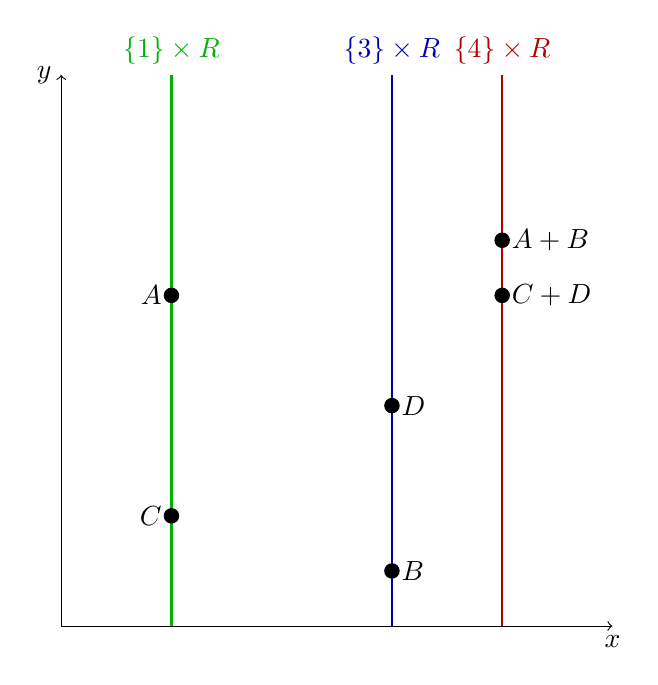
\begin{tikzpicture}[scale=1.4] 
        % Ejes
        \draw[->] (0,0) -- (5,0) node[anchor=north] {$x$};
        \draw[->] (0,0) -- (0,5) node[anchor=east] {$y$};
        
        % Líneas verticales
        \draw[green!70!black, thick] (1,0) -- (1,5) node[above] {\textcolor{green!70!black}{$\{1\} \times \mathbb{R}$}};
        \draw[blue!70!black, thick] (3,0) -- (3,5) node[above] {\textcolor{blue!70!black}{$\{3\} \times \mathbb{R}$}};
        \draw[red!70!black, thick] (4,0) -- (4,5) node[above] {\textcolor{red!70!black}{$\{4\} \times \mathbb{R}$}};
        
        % Puntos circulares
        \fill[black] (1,3) circle (2pt) node[left] {\textcolor{black}{$A$}};
        \fill[black] (1,1) circle (2pt) node[left] {\textcolor{black}{$C$}};
        \fill[black] (3,2) circle (2pt) node[right] {\textcolor{black}{$D$}};
        \fill[black] (3,0.5) circle (2pt) node[right] {\textcolor{black}{$B$}};
        \fill[black] (4,3.5) circle (2pt) node[right] {\textcolor{black}{$A+B$}};
        \fill[black] (4,3) circle (2pt) node[right] {\textcolor{black}{$C+D$}};
    \end{tikzpicture}
    \caption{\label{dibujo_cociente} Proyectar al eje horizontal puede verse como un cociente. Las clases laterales son rectas verticales.}
    \end{figure}

Ahora afirmamos que cada clase lateral de $\faktor{\mathbb{R}^2}{I}$ tiene exactamente un elemento de la forma $(a, 0)$. En efecto, primero notemos que, para todos $a, b \in \mathbb{R}$, los elementos $(a, b)$ y $(a, 0)$ están en la misma clase lateral, pues $(a, b) = (a, 0) + (0, b)$, y $(0, b) \in I$. Por otro lado, si $(a, 0)$ y $(a', 0)$ estuviesen en la misma clase lateral para algunos $a, a' \in \mathbb{R}$, entonces tendríamos que $(a-a', 0) \in I$, y eso solo es posible si $a = a'$. Por lo tanto, tenemos el isomorfismo $\left(\faktor{\mathbb{R}^2}{I}, +, \cdot\right) \simeq (\mathbb{R}, +, \cdot)$ dado por $(a, 0) + I \mapsto a$.

Geométricamente, las clases laterales corresponden a rectas verticales (ver la ilustración \ref{dibujo_cociente}). El cociente, entonces, es el conjunto de las rectas verticales, que naturalmente está en biyección con el eje horizontal. De hecho, otra forma de pensar en este cociente es que estamos proyectando el plano hacia ese eje horizontal. El hecho de que dicho cociente forme un anillo corresponde al hecho de que tomar proyecciones preserva las operaciones de suma y multiplicación cooordenada a coordenada.
\hfill$\blacksquare$
\end{example}

\begin{remark} \label{1_en_ideal}
En la definición \ref{def_ideal} es importante notar que no requerimos que $\1 \in I$. De hecho, si $I$ es un ideal que contiene al $\1$, entonces la propiedad absorbente implica que $I = R$, ya que $a = a \cdot \1$ para todo $a \in R$. Esto se condice con el hecho de que, si $\1 \in I$, entonces $\0 + I = \1 + I$ como clases laterales, lo que implicaría que el cociente $\faktor{R}{I}$ consiste de un solo elemento por la observación \ref{obs_cero_distinto_a_uno}.
\hfill$\blacksquare$
\end{remark}

\begin{example}
Dado cualquier anillo conmutativo $(R, +, \cdot)$, tenemos que $\{\0\}$ y $R$ son ideales, llamados \emph{ideales triviales}. El cociente sobre el primero es isomorfo al mismo anillo $(R, +, \cdot)$, y el cociente sobre el segundo es un anillo con un solo elemento, como mencionamos en la observación \ref{1_en_ideal}.
\hfill$\blacksquare$
\end{example}

La siguiente proposición nos da una forma sencilla de construir ideales.

\begin{prop} \label{ideal_generado}
Sea $(R, +, \cdot)$ un anillo conmutativo, y sean $a_1, a_2, \dots, a_n$ elementos de $R$. El siguiente conjunto\footnote{Hacemos notar que esta notación puede ser confusa, pues coincide con la de tuplas. En general, debiese ser claro por contexto si la notación se refiere a una tupla o al conjunto definido aquí.} es un ideal: $$\gen{a_1, \dots, a_n} \coloneqq \{r_1 \cdot a_1 + r_2 \cdot a_2 + \cdots + r_n \cdot a_n \; \mid \; r_1, r_2, \dots, r_n \in R\}.$$
\end{prop}

\begin{proof}
Veamos primero que $\gen{a_1, \dots, a_n}$ es un grupo abeliano con la suma. La asociatividad y conmutatividad se heredan directamente. Verifiquemos los tres axiomas restantes:
\begin{itemize}
\item Sean $b, c \in \gen{a_1, \dots, a_n}$. Entonces existen $r_1, \dots, r_n, s_1, \dots, s_n \in R$ tales que $b = r_1 \cdot a_1 + \cdots + r_n \cdot a_n$ y $c = s_1 \cdot s_1 + \cdots + s_n \cdot a_n$. Entonces
$$b + c = (r_1 + s_1) \cdot a_1 + (r_2 + s_2) \cdot a_2 + \cdots + (r_n + s_n) \cdot a_n,$$
por lo que $b + c \in \gen{a_1, \dots, a_n}$, y $\gen{a_1, \dots, a_n}$ es cerrado bajo la suma.
\item Usando la proposición \ref{propiedad absorbente}, tenemos que $\0 = \0 \cdot a_1 + \0 \cdot a_2 + \cdots + \0 \cdot a_n$, así que $\0 \in \gen{a_1, \dots, a_n}$.
\item Sea $b \in \gen{a_1, \dots, a_n}$, de modo que existen $r_1, \dots, r_n \in R$ tales que $b = r_1 \cdot a_1 + \cdots + r_n \cdot a_n$. Por la propiedad 1 de la proposición \ref{propiedades_anillos} tenemos que $$-b = ( - (r_1 \cdot a_1)) + ( - (r_2 \cdot a_2)) + \cdots + ( - (r_n \cdot a_n))= (-r_1) \cdot a_1 + (-r_2) \cdot a_n + \cdots + (-r_n) \cdot a_n.$$ Luego $-b \in \gen{a_1, \dots, a_n}$, y $\gen{a_1, \dots, a_n}$ es cerrado bajo tomar inversos aditivos.
\end{itemize} 
Nos falta ver que $\gen{a_1, \dots, a_n}$ es absorbente con la multiplicación. Sea $b \in \gen{a_1, \dots, a_n}$, y sea $s \in R$ arbitrario. Sabemos que existen $r_1, \dots, r_n \in R$ tales que $b = r_1 \cdot a_1 + \cdots + r_n \cdot a_n$. Luego
$$s \cdot b = (s \cdot r_1) \cdot a_1 + (s \cdot r_2) \cdot a_2 + \cdots + (s \cdot r_n) \cdot a_n,$$
por lo que $s \cdot b \in \gen{a_1, \dots, a_n}$, y $\gen{a_1, \dots, a_n}$ es absorbente. 
\end{proof}

\begin{definition}[Ideal generado, ideal principal]
Sea $(R, +, \cdot)$ un anillo conmutativo, y sean $a_1, \dots, a_n$ elementos de $R$. El ideal $\gen{a_1, \dots, a_n}$ descrito en la proposición \ref{ideal_generado} se llama el \emph{ideal generado} por los elementos $a_1, \dots, a_n$. En particular, a los ideales generados por un solo elemento se les llama \emph{ideales principales}.
\end{definition}

\begin{example} \label{modulo_n}
Veamos de nuevo el ejemplo \ref{mZ_ideal}. Notemos que, en el anillo $(\mathbb{Z}, +, \cdot)$, $m\mathbb{Z}$ es el ideal principal generado por el entero positivo $m$. Ya sabíamos que el cociente $\faktor{\mathbb{Z}}{m\mathbb{Z}}$ es isomorfo a $(\mathbb{Z}_m, +)$ como grupo abeliano (proposición \ref{isomorfismo_Z_m}). Si miramos con atención la proposición \ref{anillo_cociente}, notaremos que, de hecho, el anillo cociente\footnote{Nuevamente, aquí estamos usando usando la notación $\faktor{\mathbb{Z}}{m\mathbb{Z}}$ para referirnos al mismo tiempo a un grupo abeliano y a un anillo conmutativo. Si bien esta diferencia debe quedar clara por contexto, hacemos notar que la estructura de grupo abeliano es la que se obtiene simplemente ignorando la operación de multiplicación en la estructura de anillo conmutativo.} $\faktor{\mathbb{Z}}{m\mathbb{Z}}$ también tiene la misma estructura multiplicativa que el anillo $(\mathbb{Z}_m, +, \cdot)$. Rercordemos que este último anillo consiste de la suma y multiplicación usuales, salvo que estas se hacen en módulo $m$. Es decir, ver el cociente por el ideal principal de $m$ corresponde a ver las operaciones del anillo en módulo $m$. Esa será la noción algebraica más importante para entender este documento. \hfill$\blacksquare$
\end{example}

Notemos que el ideal $I$ del ejemplo \ref{ejemplo_cociente_R2} es también un ideal principal, generado por el elemento $(0, 1)$. De hecho, cualquier elemento $(0, b)$ con $b \neq 0$ generará el mismo ideal. En general, es común que un mismo ideal sea generado por varios conjuntos distintos de elementos del anillo.

Antes de terminar esta sección, introduciremos una notación que usaremos constantemente.

\begin{definition}[Notación de módulo] \label{notacion_modulo}
Sea $(R, +, \cdot)$ un anillo conmutativo, y sea $I \subseteq R$ un ideal. Dados $a, b \in R$, escribiremos
$$a \equiv b \modu I$$
cuando $a + I = b + I$, es decir, cuando se tenga la igualdad en el cociente. \hfill$\blacksquare$
\end{definition}

La notación de la definición \ref{notacion_modulo} generaliza la notación usual de aritmética modular. Por ejemplo, como vimos en el ejemplo \ref{modulo_n}, decir que $9 \equiv 2 \modu (7)$ corresponde a decir que los enteros $2$ y $9$ coinciden cuando consideramos el cociente sobre $7\mathbb{Z}$, el ideal generado por $7$.

\subsection{Anillos de polinomios}

\begin{definition}[Polinomios en una indeterminada, coeficientes] \label{def_polinomio}
Sea $(R, +, \cdot)$ un anillo conmutativo. Un \emph{polinomio} en la indeterminada $X$ y con coeficientes en $R$ es una expresión formal de la forma
$$p(X) = a_0 + a_1X + a_2X^2 + \cdots + a_n X^n,$$
donde $n$ es un entero no negativo y $a_0, a_1, \dots, a_n \in R$. Se dice que $a_0, a_1, \dots, a_n$ son los \emph{coeficientes} de $p(X)$.

Al conjunto de todos los polinomios en la indeterminada $X$ y con coeficientes en $R$ lo denotamos $R[X]$. 
\hfill$\blacksquare$
\end{definition}

En la definición \ref{def_polinomio}, <<expresión formal>> significa que un polinomio no debe entenderse \textit{a priori} como una función, sino como un objeto en sí mismo. En ese sentido, las distintas potencias de $X$ solo sirven para separar los coeficientes. De hecho, podríamos haber definido los polinomios con coeficientes en $R$ simplemente como tuplas $(a_0, a_1, \dots, a_n)$ de elementos de $R$. Las razones por las que se prefiere la primera notación quedarán claras a medida que avancemos en esta sección.

El orden en el que se escriben los términos $a_k X^k$ es irrelevante. Usualmente se omiten aquellos con $a_k=\0$, y simplemente se escribe $X^k$ cuando $a_k = \1$.

\begin{definition}[Grado, polinomio nulo, polinomio constante]
Sea $R$ un anillo conmutativo, y consideremos un polinomio $p(X) \in R[X]$. Digamos que
$$p(X) = a_0 + a_1X + a_2X^2 + \cdots + a_n X^n.$$
El \emph{grado} de $p(X)$, denotado $\mathrm{gr}(p(X))$, es el mayor entero no negativo $m$ tal que $a_m \neq \0$. Si dicho entero no existe, es decir, si todos los coeficientes de $p(X)$ son iguales a $\0$, entonces definimos $\mathrm{gr}(p(X)) = -\infty$, en cuyo caso a $p(X)$ lo llamamos \emph{polinomio nulo} y escribimos $p(X) = \0(X)$. Por otro lado, si $\mathrm{gr}(p(X)) = 0$, es decir, si $p(X) = a_0$, decimos que $p(X)$ es un \emph{polinomio constante}.
\hfill$\blacksquare$
\end{definition}

Uno puede definir la suma y multiplicación de polinomios en $R[X]$ de la manera usual, con la salvedad de que los coeficientes deben operarse según la suma y multiplicación del anillo $R$. Dejamos como ejercicio para el lector verificar que, para cualquier anillo conmutativo $R$, $R[X]$ forma un anillo con estas operaciones. El polinomio nulo es el neutro aditivo, y el inverso aditivo de $p(X)$ se obtiene tomando el inverso aditivo de cada coeficiente. La identidad es el polinomio constante igual a $\1$.

\begin{example}
Consideremos los polinomios 
$$p(X) = 2X^2 + 3X + 4 \quad , \quad q(X) = 4X^3 + X^2 \quad , \quad r(X) = 2X^4 + 3X^3 + X^2 + 3$$
en el anillo de polinomios $\mathbb{Z}_5[X]$. Tenemos que
\begin{align*}
(p(X) \cdot q(X)) + r(X) &= \left((2 \cdot 4)X^5 + (2 \cdot 1 + 3 \cdot 4)X^4 + (3 \cdot 1 + 4 \cdot 4)X^3 + (4 \cdot 1)X^2 \right) + r(X) \\
&= (3X^5 + 4X^4 + 4X^3 + 4X^2) + (2X^4 + 3X^3 + X^2 + 3) \\
&= 3X^5 + (4 + 2)X^4 + (4 + 3)X^3 + (4 + 1)X^2 + 3 \\
&= 3X^5 + X^4 + 2X^3 + 3.
\end{align*}
\hfill$\blacksquare$


\end{example}